\chapter{Results}
\label{chap:results}

In this chapter the results of the GraphSLAM algorithm are presented for different test scenarios. In section~\ref{sec:known-asso-res} the algorithm is tested for the simple case of known data association and simulated data. A parameters variation analysis is made, and their effect in the path estimation is shown. In section~\ref{sec:unknown-asso-res} a similar analysis is performed, but for the case of unknown data association. In this case, new parameters related to de data association algorithm are tested. Finally in section~\ref{sec:real-data-res}, the GraphSLAM algorithm is run in more realistic data. This data includes robot simulated with Gazebo\footnote{http://gazebosim.org/}, a much more realistic robot simulator, and data obtained from real robots in outdoor environments. 

Through this tests several parameters and methods must be chosen for the algorithm to work properly. To limit the scope of this work, the sparse solver and the optimization algorithm are fixed and used in all the following tests. CSpase library and the Cholesky decomposition s use for the sparse solver, and the Levenberg-Marquardt method is used as the optimization algorithm. Also whenever the robust kernel method is used, Huber is the chosen kernel function (see subsection~\ref{sec:known-asso-imp}). 

\section{Known Data Association}
\label{sec:known-asso-res}

The known data association case is the easiest one of the three scenarios, because correspondence between landmarks is given a priori. In this case he user must simply set the parameters and run the solver as stated in algorithm~\ref{alg:known-correspondence}. 

The parameters to be set in this test are the following:

\begin{itemize}
    \item $n_p$: number of poses in the robot path.
    \item $n_l$: number of landmarks in the map.
    \item $i_{op}$: odometry position information (inverse of variance).
    \item $i_{oa}$: odometry angle information.
    \item $i_{lp}$: landmark position information.
    \item $it$: number of iterations for the optimization algorithm to stop.
    \item $k_w$: Width of the chosen robust kernel.
\end{itemize}

Where $n_p$, $n_l$, $i_{op}$, $i{oa}$, and $i_{lp}$ are parameters regarding the robot behavior in the test, and passed to the simulator. The parameters $it$ and $k_w$ define de optimization strategy.

Through all the test made in this work, it is assumed that the information matrix of odometry and measurements models (same as~\eqref{eq:info-matrices}) are diagonal, i.e., their variables are not correlated. Furthermore, it is assumed that these matrices have the following structure:

\begin{equation}
\bs{R}^{-1}_k = \begin{pmatrix}
i_{op} & 0 & 0\\
0 & i_{op} & 0\\
0 & 0 & i_{oa}
\end{pmatrix} \;\;
\bs{Q}^{-1}_k = \begin{pmatrix}
i_{lp} & 0\\
0 & i_{lp}
\end{pmatrix} 
\label{eq:info-matrices-tests}
\end{equation}

This means that the robot experiences same uncertainty in the $x$ and $y$ axis, for both models. 

\begin{test}

The first test is run with the parameters of Table~\ref{tab:test-i}. 

The simulation is constrained to a 2D world with $x\in[-25,25]$, $y\in[-25,25]$. At each step the simulator moves the robot 1 unit of distance and in turns randomly an angle of $\theta=0^\circ$, $90^\circ$, or $-90^\circ$. All simulations start from at $(0,0)$.

A kernel width of 1 unit is chosen heuristically, looking at the distance between landmarks. 

The results of the test are shown in Figure~\ref{fig:test-i}. In Figure~\ref{fig:test-ia} the initial guess of the solver is plotted on the left, and the posterior estimation after the solver on the right. The groundtruth is added in both graphs for comparison. Note that not necessarily are observed.  It can be seen that the path of the initial guess rapidly diverges from the real solution. On the other hand, the solver estimation fits quite well with the groundtruth, both for the path and the landmarks.

To have a more quantitative view of the error made by the solver, the cumulative path error for every step is shown in Figure~\ref{fig:test-ib}.  The cumulative normalized error is given by:

\begin{equation}
error (i) = \frac{1}{i} \sum_{i} ||pos_{GT}-pos_{est}||
\end{equation} 

Where $i$ is the path's timestep. $pos_{GT}$ and $pos_{est}$ are the groundtruth and estimated position respectively. then the error is the sum of the euclidean distance of both positions, normalized by the number of steps. 

It can be seen that the error start increasing early in the path, but then it get stabilized. This is the effect of aggregating the information of the measurements and running the optimizer. as long as the robot keep measuring repeated landmarks, it can maintain its error low. 

\begin{table}[htbp!]
\centering
\begin{tabular}{|c|c|c|c|c|c|c|}
    \hline
    $n_p$ & $n_l$ & $i_{op}$ & $i_{oa}$ & $i_{lp}$ & $it$ & $k_w$\\
    \hline \hline
    300 & 40 & 1000 & 1000 & 1000 & 20 & 1\\
    \hline 
\end{tabular}
\caption{Parameters for Test~\Roman{test}.}
\label{tab:test-i}
\end{table}

\begin{figure}[htbp!]
    \centering
    \begin{subfigure}[b]{0.8\textwidth}
        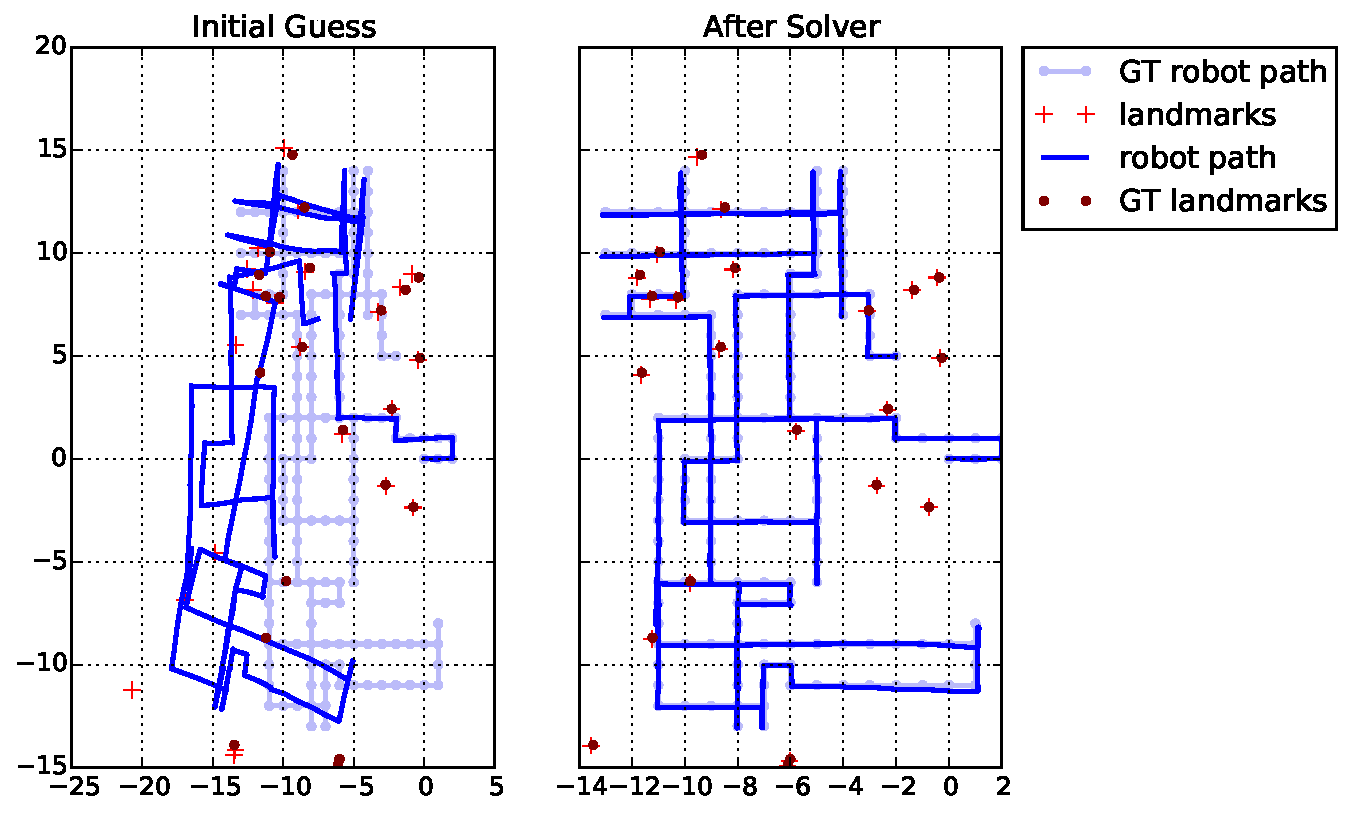
\includegraphics[width=\textwidth]{imagenes/tests/known/res_nl_40_op_1000_oa_1000_lp_1000_ds_300_nl_40_op_1000_oa_1000_lp_1000_ds_300.pdf}
        \caption{Initial guess and solver estimation.}
        \label{fig:test-ia}
    \end{subfigure}\\
    \begin{subfigure}[b]{0.6\textwidth}
        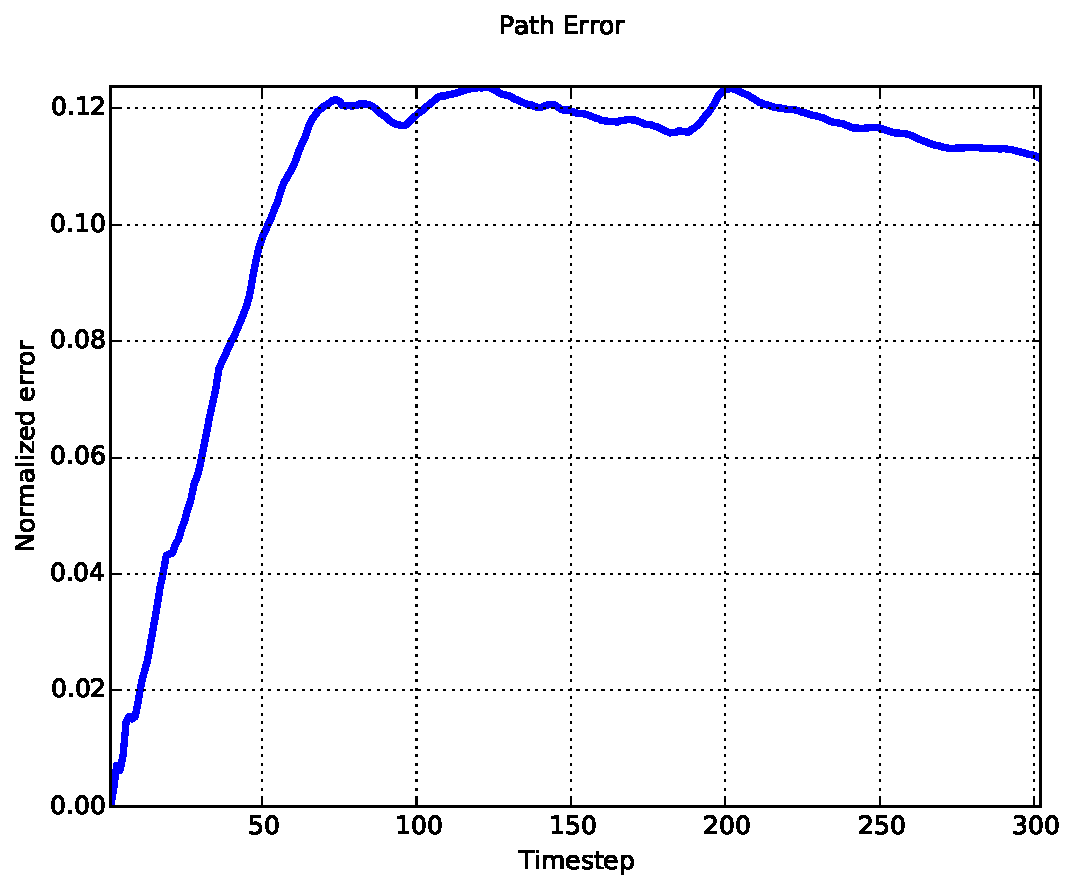
\includegraphics[width=\textwidth]{imagenes/tests/known/res_nl_40_op_1000_oa_1000_lp_1000_ds_300_nl_40_op_1000_oa_1000_lp_1000_ds_300_path.pdf}
        \caption{Path normalized error.}
        \label{fig:test-ib}
    \end{subfigure}
    \caption{Results for Test~\Roman{test}.}
    \label{fig:test-i}
\end{figure}

\end{test}

\section{Unknown Data Association}
\label{sec:unknown-asso-res}

\section{Real Data}
\label{sec:real-data-res}